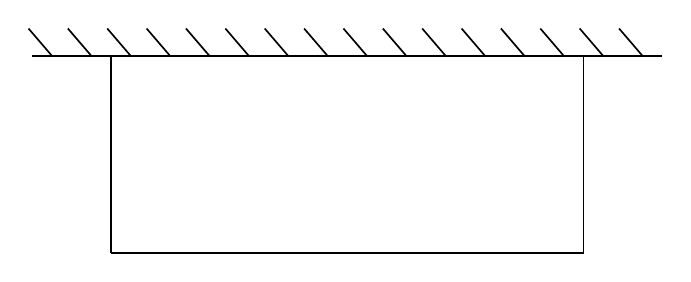
\begin{tikzpicture}[x=1cm,y=1cm,line width=.6pt,font=\normalsize]
% wall
\draw (-1.0,2.5) -- (7.0,2.5);
% hatch ticks above wall
\foreach \x in {-0.75,-0.25,0.25,0.75,1.25,1.75,2.25,2.75,3.25,3.75,4.25,4.75,5.25,5.75,6.25,6.75} {
  \draw (\x,2.5) -- ++(-0.30,0.35);
}
% fence: left / bottom / right (top coincides with wall segment, no labels in source)
\draw (0.0,0.0) -- (0.0,2.5);
\draw (0.0,0.0) -- (6.0,0.0);
\draw (6.0,0.0) -- (6.0,2.5);
\end{tikzpicture}
